\newpage
\section{Progetto di reti logiche combinatorie}
\begin{definition}[Circuito]
	Un \textbf{circuito} è una rete elettrica che elabora variabili a valori discreti.
\end{definition}
Un circuito contiene:
\begin{itemize}
	\item Uno o più \textbf{ingressi} a valori discreti
	\item Una o più \textbf{uscite} a valori discreti
	\item Una \textbf{specifica funzionale} che descrive la relazione tra ingressi e uscite
	\item Una \textbf{specifica temporizzazione} che descrive il ritardo tra il cambio degli ingressi e la risposta delle uscite
\end{itemize}
\begin{center}
	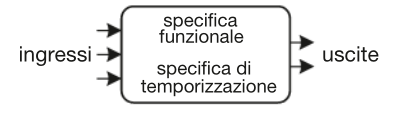
\includegraphics[scale=0.4]{circuito.png}
\end{center}
All'interno è composta da \textbf{elementi}, ovvero a loro volta reti logiche, e \textbf{nodi}, ovvero contatti elettrici la cui tensione trasmette un valore discreto. Questi si dividono in:
\begin{itemize}
	\item \textbf{Ingressi}: ricevono valori dal mondo esterno
	\item \textbf{Uscite}: emettono valori all'esterno
	\item \textbf{Interni}: tutti gli altri
\end{itemize}
\begin{center}
	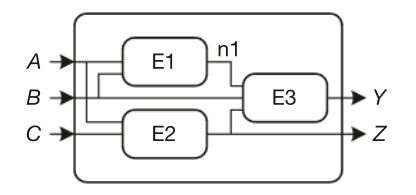
\includegraphics[scale=0.3]{nodes.png}
\end{center}

Le reti digitali vengono divise in:
\begin{itemize}
	\item \textbf{Combinatorie}: le uscite dipendono esclusivamente dai valori presenti in ingresso
	\item \textbf{Sequenziali}: le uscite dipendono sia dai valori di ingresso sia da quelli precedenti. è quindi dotata di \textbf{memoria}
\end{itemize}

\subsection{Mappe di Karnaugh}
Per semplificare le espressioni booleane usate per rappresentare le reti, è possibile usare le mappe di Karnaugh. A partire dalla tabella di verità, si costruisce un'altra tabella che ha come righe e colonne tutte le possibili combinazioni dei letterali ordinate tramite il \textbf{codice Gray}, ovvero ogni combinazione adiacente deve differire solo per un letterale.
\begin{center}
	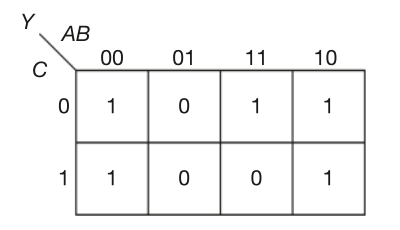
\includegraphics[scale=0.4]{k-map_1.png}
\end{center}
\newpage
Si costruiscono poi dei \textit{cerchi} che devono:
\begin{itemize}
	\item Essere in numero minore possibile
	\item Tutti i riquadri devono contenere $1$
	\item Ogni cerchio deve includere un numero di riquadri che sia una potenza di $2$
	\item Ogni cerchio deve essere il più grande possibile
	\item Si possono disegnare cerchi che vanno dalla fine della mappa all'inizio (pac-man effect)
	\item Un riquadro può essere cerchiato più di una volta
\end{itemize}
Una volta costruiti i cerchi, per ognuno di essi creiamo un termine della nostra espressione semplificata: ogni termine avrà i letterali che non cambiano tra i riquadri cerchiati e non avrà quelli che cambiano. Questo perché se un termine cambia ma il risultato rimane $1$, vuol dire che non è utile (\textbf{indifferenza}).
\begin{center}
	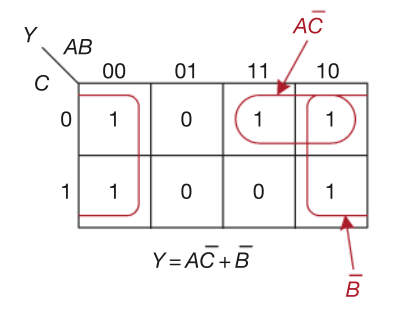
\includegraphics[scale=0.4]{k-map_2.png}
\end{center}

\subsection{Blocchi costruttivi}
\subsubsection{Multiplexer}
Permettono di scegliere un'uscita a partire da un certo numero di ingressi possibili basandosi sul valore di un \textbf{segnale di controllo}.
\begin{center}
	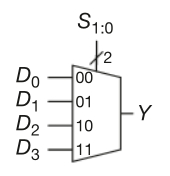
\includegraphics[scale=0.4]{mux.png}
\end{center}
Possono essere utilizzati come \textbf{lookup table} per eseguire funzioni logiche.
\begin{center}
	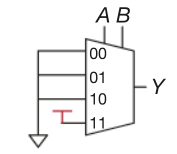
\includegraphics[scale=0.3]{mux_lookup.png}
\end{center}
È possibile ridurre il numero di ingressi da $2^N$ a $2^{N-1}$, fornendo uno dei letterali in ingresso come segnale di controllo.
\begin{center}
	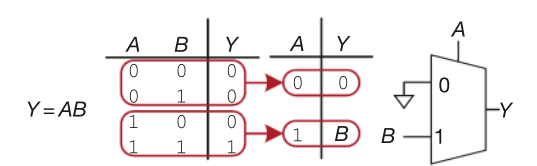
\includegraphics[scale=0.3]{mux_small.png}
\end{center}
\subsubsection{Decoder}
Ha $N$ ingressi e $2^N$ uscite e attiva una di queste in base alla combinazione dei valori in ingresso.
\begin{center}
	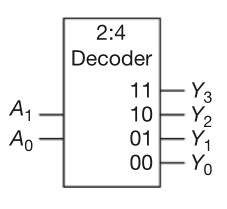
\includegraphics[scale=0.4]{demux.png}
\end{center}
Possono essere utilizzati assieme a delle porte \textit{OR} per costruire funzioni logiche. In particolare una funzione ad $N$ ingressi e $M$ uni nella tabella di verità, si può rappresentare con un decoder $N:2^N$ e con una porta \textit{OR} a $M$ ingressi.
\begin{center}
	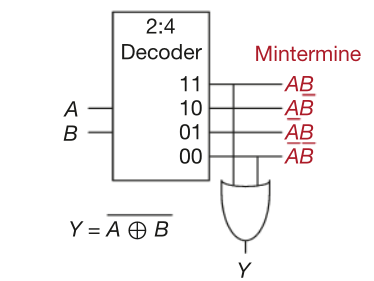
\includegraphics[scale=0.3]{denux_logic.png}
\end{center}

\subsection{Temporizzazioni}
Uno dei problemi più importanti delle reti è come fare in modo che queste funzioni velocemente.\\
Il \textbf{diagramma temporale} rappresenta la \textbf{risposta transitoria} della rete al cambiare di un ingresso. Ci sono due sezioni:
\begin{itemize}
	\item Fronte di \textbf{salita}: passaggio da \textit{BASSO} ad \textit{ALTO}
	\item Fronte di \textbf{discesa}: passaggio da \textit{ALTO} a \textit{BASSO}
\end{itemize}
\begin{center}
	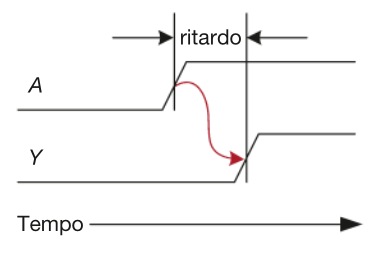
\includegraphics[scale=0.3]{ritardi.png}
\end{center}
\subsubsection{Ritardi}
Esistono due tipi di ritardi:
\begin{itemize}
	\item \textbf{Propagazione}, $t_{pd}$: il tempo massimo che trascorre dal cambiamento di un ingresso al momento in cui l'uscita raggiunge il valore finale
	\item \textbf{Contaminazione}, $t_{cd}$: il tempo minimo che trascorre dal momento in cui cambia un ingresso al momento in cui una qualsiasi uscita comincia il processo di adattamento del suo valore
\end{itemize}
\begin{center}
	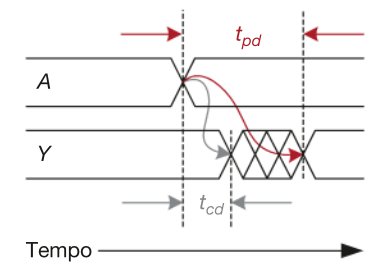
\includegraphics[scale=0.3]{ritardi_tipi.png}
\end{center}

\begin{note}
	Le cause del ritardo includono il tempo richiesto per caricare in una rete e la velocità della luce. Inoltre, i due tipi di ritardi possono essere diversi per:
	\begin{itemize}
		\item Diversi ritardi tra salita e discesa
		\item Ingressi e uscite multipli, alcuni più veloci di altri
		\item Reti che rallentano al surriscaldamento e si velocizzano al raffreddamento
	\end{itemize}
\end{note}
Il valore dei ritardi è determinato anche dal \textbf{percorso critico}, ovvero il percorso seguito dal segnale tra l'ingresso e l'uscita. Il \textbf{percorso minimo} è invece quello più breve possibile.
\begin{center}
	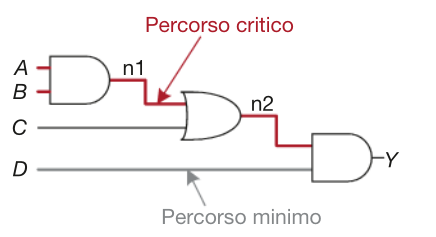
\includegraphics[scale=0.3]{delay_path.png}
\end{center}
In una rete il ritardo di propagazione è uguale alla somma dei singoli ritardi di ogni elemento del percorso critico, mentre il ritardo di contaminazione è la somma dei ritardi di contaminazione di ogni elemento del percorso minimo.
\begin{align}
	& t_{pd} = 2t_{pd\_AND} + t_{pd\_OR} \\
	& t_{cd} = t_{cd\_AND}
\end{align}

\subsubsection{Alee}
È possibile che un cambiamento singolo in ingresso possa causare più cambiamenti in uscita indesiderati: le \textbf{alee}.\\
Non rappresentano un problema se si aspetta che il ritardo di \textit{propagazione} si sia esaurito prima di guardare il valore di uscita poiché questa prima o poi torna sul risultato corretto.\\
Si può evitare aggiungendo un'altra porta facendo riferimento alla mappa di Karnaugh. È sufficiente aggiungere un cerchio quando il cambio di una variabile "attraversa" due cerchi adiacenti (con un costo maggiore a livello HW).
\begin{center}
	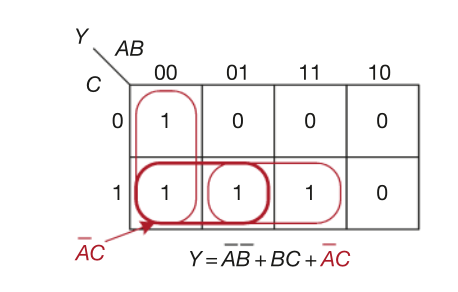
\includegraphics[scale=0.3]{alee.png}
\end{center}